\chapter{Arbejdsblade}

\section{Sygdom}\label{symp}
Hjertesvigt beskriver en tilstand hvor hjertemusklen er svækket og hjertets pumpeevne ikke er tilstrækkelig til at imødekomme kroppens behov \citep{TSchroeder20160}. Prævalensen er stigende, da befolkningen bliver ældre, og behandlingen af akutte hjerte-kar-sygdomme er blevet bedre \citep{heartfailure}.\\
Hjertesvigt er et syndrom karakteriseret ved symptomer som åndenød, hævede ankler og træthed, og fund som øget halsvenetryk, krepetitioner i lungerne og perifere ødemer, der skyldes struktureller eller funktionelle abnormaliteter i hjertet, der fører til øget intrakardialt tryk eller et reduceret cardiac output ved hvile eller under stress. Overordnet kan hjertesvigt inddeles i kronisk og akut. Akut hjertesvigt defineres som symptomer og fund på hjertesvigt, der opstår pludseligt og kræver akut behandling, hvorimod kronisk hjertesvigt opstår over længere tid, og hvor hospitalsbesøg er planlagte. I det følgende fokuseres på kronisk hjertesvigt, da det som beskrevet i indledningen er disse der monitoreres.\citep{heartfailure}\\
Kronisk hjertesvigt påvirker omkring 2\% af den voksne befolkning på verdensplan. Prævalensen afhænger i høj grad af alderen, og er mindre end 2\% for personer under 60 år, og mere end 10\% for personer over 75 år. Patienter med hjertesvigt har en dårlig prognose med mange hospitalsindlæggelser og høj mortalitet på 6-7\% per år.\citep{heartfailure}\\
\\
Der er overordnet to forskellige typer af hjertesvigt; systolisk og diastolisk hjertesvigt. Systolisk hjertesvigt er en tilstand med dilateret ventrikel, som medfører en nedsat pumpekraft og dermed nedsat evne til at opretholde minutvolumen, blodtryk og tilstrækkelig perifer cirkulation. Diastolisk hjertesvigt definerer en tilstand med nedsat fyldning af ventriklerne pga. nedsat eftergivelighed i ventriklen.\citep{TSchroeder2016}\\
Hjertesvigt kan være venstresidigt, højresidigt eller en kombination af begge og giver forskellige symptomer alt afhængig af hvilket område af hjertet der er påvirket. Ved venstresidigt svigt er det vanskeligt for hjertet at pumpe blodet videre fra lungekredsløbet og der kan opstå lungeødem. Dette kan give symptomer som dyspnø som forværres ved fysisk aktivitet. Ved højresidigt svigt er det vanskeligt for hjertet at pumpe det afiltede blod tilbage til lungerne og blodet ophobes i kroppen som kan føre til ødemer i resten af kroppen f.eks. benene. \cite{TSchroeder2016}\\
Hjertesvigt forekommer som resultat af en myokardiskade eller længevarende belastning af myorkardiet, hvilket medfører ændringer i hjertets struktur og geometri. Dette kan eksempelvis skyldes iskæmi eller ardannelse efter et myokardiinfarkt, ventrikelhypertrofi pga. hypertension eller aortastenose, hjerteklapsygdomme eller toksisk myokardipåvirkning f.eks. ved længevarende alkoholindtag  eller kemoterapi. For at kompensere for den nedsatte pumpefunktion igangsættes nogle mekanismer for at opretholde mængden af blod som cirkulerer rundt i kroppen. Her kan blandt andet nævnes at hjertets slagvolumen øges, strukturen af hjertemusklen ændres i form af dilation og hypertrofi, der sker en aktivering af det sympatiske nervesystem og renin-angiotensin-aldosteron-systemet. På kort sigt vil de kompensatoriske mekanismer øge cardiac output men på længere sigt vil det belaste hjertet yderligere, hvorved tilstanden forværres.\citep{TSchroeder2016}\\
Den øgede belastning på hjertet forekommer som resultat af en øget pre- og afterload. Aktivering af det sympatiske system øger hjertefrekvensen og  kontraktiliteten, hvilket fører til en øget afterload. Aktivering af renin-angiotensin-aldosteron-systemet medfører væske- og natriumretention, hvilket bidrager til ventrikeldilation og medfører yderligere belastning ved at hæve hjertets preload. Disse processer fører til et øget iltforbrug i myokardiet som ikke kan kompenseres for og vil på længere sigt føre til myocytnekrose. Dette resulterer i at slagvolumen nedsættes yderligere og den onde cirkel gentager sig igen.\citep{TSchroeder2016}

\subsection{Klassificering af hjertesvigt}
Der bruges flere systemer til at klassificere hjertesvigt, der er baseret på enten symptomer eller progression. 

\begin{itemize} 
\item NYHA I: Der opleves ingen symptomer eller begrænsninger under almindelig fysisk aktivitet.
\item NYHA II: Der opleves ingen symptomer under hvile eller under lettere fysisk aktivitet, men lav grad af åndenød, træthed, hjertebanken ved moderat fysisk aktivitet som trappegang til 2. sal, havearbejde, støvsugning, bære tunge ting.
\item NYHA III:  Ingen symptomer i hvile, men blot ved let fysisk aktivitet som påklædning eller gang i fladt terræn giver udmattelse, åndenød, evt. hjertebanken eller brystsmerter.
\item NYHA IV: Der opleves symptomer i hvile, som forværres ved fysisk aktivitet
\end{itemize}

% , se figur \ref{fig:ondcirkel}. \cite{TSchroeder2016}

%\begin{figure}[H]
%\centering
%  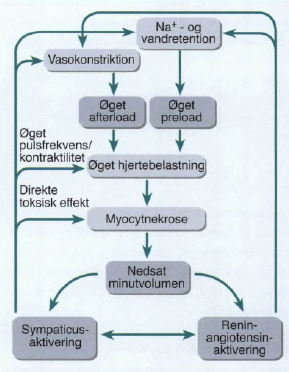
\includegraphics[width=0.4\textwidth]{Billeder/ondcirkel.png}
%   \caption{Ved hjertesvigt aktiveres sympaticus og renin-angiotensin-aldosteron-systemet som på længere sigt vil øge hjertebelastningen og forværre tilstanden \cite{TSchroeder2016}.} 
%   \label{fig:ondcirkel}
%\end{figure}

\section{Diagnose}
Da sen diagnose af hjertesvigt giver en øget mortalitet, er det vigtigt at diagnosticere patienter tidligt og få dem i tidlig behandling. I løbet af behandlingsforløbet skal patienter til rutinemæssige kontrol hos egen læge for at sikre at sygdommen ikke forværres og at patienten dermed får den rette behandling. \cite{heartfailure}

Patienter med hjertesvigt får oftest stillet diagnosen gennem kontakt med læge i forbindelse med at opleve symptomerne beskrevet i \autoref{symp}. Patienten bliver her henvist til en række undersøgelser med henblik på at undersøge hjertet. \cite{heartfailure}
Der bliver altid taget et elektrokardiogram, EKG. EKG kan foretages af primærsektoren og benyttes til at sænke eller styrke mistanken om hjertesvigt. Resultatet giver nyttige oplysninger om potentielle årsager til akut hjertesvigt og et mål for en specifik behandling. Et biokemi kontrol af blodværdier benyttes til at bestemme årsag til symptomer og hvordan behandling kommer til at forløbe. \cite{DCS}
Ekkokardiografi er essentielt i diagnosen af hjertesvigt. Undersøgelsen giver en visualisering af hjertet hvor tegn på blodprop, hjerteklap fejl kan ses og pumpefunktion kan udregnes. \cite{heartfailure}\cite{DCS}
Undersøgelsen giver hverisær årsager til symptomer hvoraf diagnosen hjertesvigt kan stilles samt i hvor svær grad hjertet er svækket. Patienter med hjertesvigt oplever bla. åndenød og inddeles herefter på skalaen NYHA, The New York Heart Association klasse, alt efter hvor svær åndenød der opleves. \cite{heartfailure}\cite{DCS}
% Diagnosen bliver stillet på baggrund af patientens sygehistorie og en række undersøgelser.

% \begin{itemize} 
% \item{Et røntgenbillede af brystkassen, giver en visualisering af lungerne og afslører hvorledes der er væske i lungerne}
% \item{Ultralydsscanning, giver en visualisering af hjertet hvor tegn på blodprop, hjerteklap fejl kan ses og pumpefunktion kan udregnes}
% \end{itemize}
% Undersøgelserne bliver ultimativt benyttet til at udelukke andre sygdomme der viser samme symptomer og samtidig specificere i hvor svær grad hjertets pumpefunktion er svækket.  
% Patienter med hjertesvigt oplever bl.a. åndenød og inddeles herefter på skalaen NYHA, The New York Heart Association klasse, alt efter hvor svær åndenød der opleves. 

\begin{itemize} 
\item NYHA I: Der opleves ingen symptomer eller begrænsninger under almindelig fysisk aktivitet.
\item NYHA II: Der opleves ingen symptomer under hvile eller under lettere fysisk aktivitet, men lav grad af åndenød, træthed, hjertebanken ved moderat fysisk aktivitet som trappegang til 2. sal, havearbejde, støvsugning, bære tunge ting.
\item NYHA III:  Ingen symptomer i hvile, men blot ved let fysisk aktivitet som påklædning eller gang i fladt terræn giver udmattelse, åndenød, evt. hjertebanken eller brystsmerter.
\item NYHA IV: Der opleves symptomer i hvile, som forværres ved fysisk aktivitet
\end{itemize}

NYHA benytte til at bestemme hvilken behandling patienten skal modtage og hvilken behandling der kan overvejes. \cite{DCS}